\subsubsection{Spezialkunststoff: CYTOP\textsuperscript{\texttrademark}}
\label{subsec:pofcytop}

CYTOP\textsuperscript{\texttrademark} (Cyclic Transparent Optical Polymer) ist
ein von Asahi Glass Company entwickeltes, vollständig fluoriertes Polymer. Der
Kunstoff verfügt über eine optische Durchlässigkeit von 95 \% und ist resistent
gegenüber organischen Lösungsmittel sowie gegenüber Säuren und Basen mit einer
Konzentration bis zu 50 \% \cite{pofagc}. \autoref{rec:cytop} zeigt die
Strukturformel von CYTOP\textsuperscript{\texttrademark}. Es handelt sich um
einen amorphen Thermoplast, der über keinerlei
Wasserstoff-Kohlenstoff-Verbindungen verfügt, sondern nur über
Fluor-Kohlenstoff-Verbindungen.

\begin{figure}[H]
    \begin{center}
        \begin{minipage}{0.4\textwidth}
            \begin{center}
                \footnotesize
                %\setatomsep{1.7em}

                \chemname{\chemfig{-[@{op,0.5}]CF_2-[7,,1,2]FC(-[:-108,,2]\lewis{35,O}-[:-36,,,1]CF_2-[:36,,1]C?[a]F_2)-C?[a]F-[1,,1,2]F_2C-[@{cl,0.5}]}}{}
                \makebraces[5pt,70pt]{n}{op}{cl}

                \caption{CYTOP\textsuperscript{\texttrademark}}
                \label{rec:cytop}
            \end{center}
        \end{minipage}
        \hspace{0.025\textwidth}
        \begin{minipage}{0.4\textwidth}
            \begin{center}
                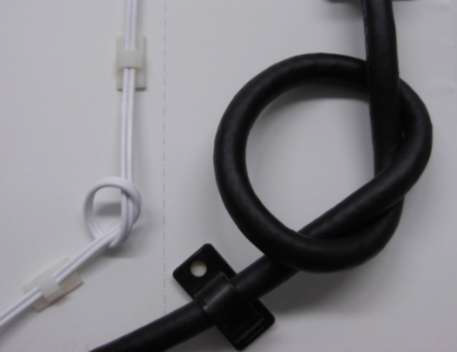
\includegraphics[height=0.1275\textheight]{Bilder/Optische_Wellenleiter_Die_Polymer_Optische_Faser/Kernmaterialien/poffontexkupfer.png}
                \caption[Links: FONTEX\textsuperscript{\texttrademark}, Rechts: Kupferkabel\newline              \url{www.lucina.jp/eg_fontex/pdf/Tecnhical.pdf} S.10 (zuletzt aufgerufen am 19.09.2015)]{Links: FONTEX\textsuperscript{\texttrademark}, Rechts: Kupferkabel}
                \label{fig:poffontexkupfer}
            \end{center}
        \end{minipage}
    \end{center}
\end{figure}

CYTOP\textsuperscript{\texttrademark} wird als Kernmaterial für die polymer
optische Faser FONTEX\textsuperscript{\texttrademark} verwendet, welche
ebenfalls von der Asahi Glass Company produziert wird.
FONTEX\textsuperscript{\texttrademark} eignet sich aufgrund hoher
Übertragungsraten, geringem Gewicht und geringem Stromverbrauch insbesondere für
den Einsatz in Rechenzentren. Außerdem ist der Platzverbrauch von
FONTEX\textsuperscript{\texttrademark} geringer und die Biegsamkeit höher als
bei Kupferkabeln (siehe \autoref{fig:poffontexkupfer}). \cite{poffontex}
